\section{Einführung}
\textbf{Mikrowellen} sind elektromagnetische Wellen mit einer Wellenlänge zwischen ca. \SI{1}{mm} und \SI{30}{cm}.\\

Gehen von einem Sender elektromagnetische Strahlen aus, so beschreibt die \textbf{Strahldivergenz} die Aufweitung des Strahlenbündels mit zunehmendem Abstand zum Sender. Sie wird angegeben durch den Winkel $\theta$ zwischen den äußersten Strahlen (bzw. dort, wo die Feldstärke auf \SI{10}{\percent} des Maximums abfällt).\\

Eine \textbf{stehende Welle} ist eine Welle mit Knotenpunkten, an denen keine Auslenkung stattfindet. Sie kann erzeugt werden durch Reflexion, wobei die reflektierte Welle sich mit der einfallenden überlagert. Der Abstand von zwei Knotenpunkten entspricht der halben Wellenlänge.\\

Trifft eine elektromagnetische Welle aus einem Medium mit Brechungsindex $n_1$ auf eine Grenzfläche zu einem Medium mit Brechungsindex $n_2$, so wird ein Teil reflektiert und ein Teil transmittiert. Die transmittierte Welle breitet sich in der durch die einfallende Welle und die Oberflächennormale auf der Grenzfläche aufgespannten Ebene aus. Die Winkel $\vartheta_1$ der einfallenden und $\vartheta_2$ der transmittierten Welle stehen über das Snelliussche Brechungsgesetz in Zusammenhang:
\begin{equation}
	n_1\sin{\vartheta_1}=n_2\sin{\vartheta_2}
\label{eq:snellius}
\end{equation}

Ist Medium 1 dichter als Medium 2, d.h. $n_1>n_2$, so steht bei einem bestimmten Einfallswinkel $\vartheta_T$ die transmittierte Welle senkrecht zur Oberflächennormalen. Dieser Winkel heißt \textbf{Grenzwinkel der Totalreflexion} und er ergibt sich aus 
\begin{equation}
	\sin{\vartheta_T}=n_2/n_1\qquad .
\label{eq:total}
\end{equation}

Wird der Einfallswinkel noch flacher, d.h. $\vartheta_1>\vartheta_T$, so wird die Welle vollständig reflektiert. Allerdings dringt die sog. evaneszente Welle in Medium 2 ein. Sie propagiert parallel zur Grenzfläche und nimmt exponentiell mit dem Abstand zu dieser ab.

Wird ein Medium 3 mit Brechungsindex $n_3$ nahe hinter Medium 2 gebracht, so erzeugt die evaneszente Welle eine Welle, die in Medium 3 propagiert. Dies nennt man \textbf{frustrierte Totalreflexion}.\\

Fällt eine elektromagnetische Welle auf eine mehrschichtige Netzstruktur (z.B. ein Kristall oder ein Gitter aus Metallkugeln), so wird sie an den verschiedenen Schichten reflektiert. Die reflektierten Wellen überlagern sich mit Phasenunterschieden, die auf die unterschiedlich langen Wege zurückzuführen sind. Die \textbf{Braggsche Reflexionsbedingung} gibt an, bei welchen Glanzwinkeln $\alpha$ die von Netzebenen mit Abstand $d$ reflektierten Wellen konstruktiv interferieren:
\begin{equation}
	2d\sin{\alpha}=n\lambda\qquad n\in\mathbb{N^+}
\label{eq:bragg}
\end{equation}

\section{Versuch}
In den Versuchen sollten die in der Einleitung beschriebenen Phänomene bei Mikrowellen untersucht werden. Dazu standen ein Mikrowellensender und ein Empfänger zur Verfügung. Über eine Spannungsquelle konnte die Sendestärke geregelt werden und mit einem Spannungsmessgerät wurde eine Spannung gemessen, die proportional zur Intensität am Empfänger war. 
\subsection{Strahldivergenz}
Um die Strahldivergenz zu bestimmen, wurde in vier verschiedenen Abständen zum Sender der Abstand zu beiden Seiten der optischen Achse bestimmt, an dem die Spannung beim Empfänger um ca. \SI{10}{\percent} vom maximalen Wert abgefallen war.
\begin{figure}[h]
\centering
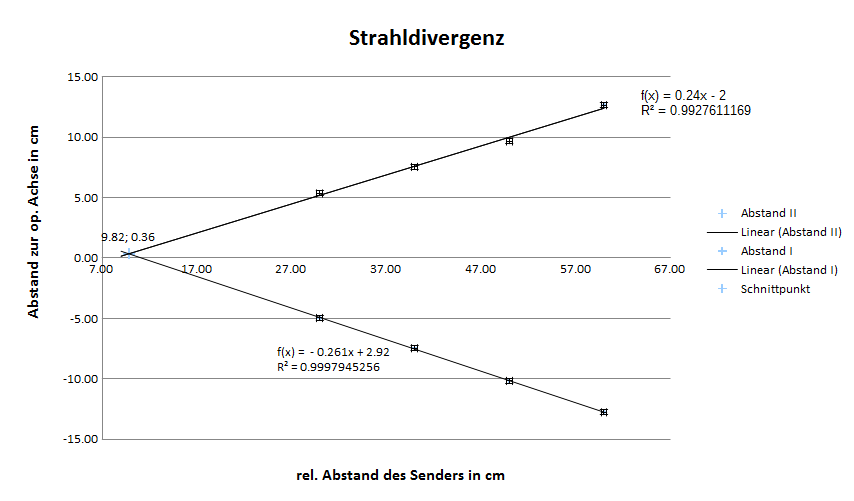
\includegraphics[width=\linewidth]{res/Nr2neu.png}
\caption{Strahlprofil des Mikrowellensenders in vier Entfernungen vom Sender bei Abfall der Empfängerspannung auf \SI{10}{\percent} des Maximalwertes.}
\label{fig:strahldiv}
\end{figure}
Mit Excel wurden je ein linearer Fit der vier Messpunkte zu beiden Seiten der optischen Achse durchgeführt. Der Öffnungswinkel errechnetet sich durch den $\arctan$ der Steigungen:
\begin{equation}
\theta=\frac{\SI{180}{\degree}}{\pi}(\arctan(\num{0.24})+\arctan(\num{0.261}))=\SI{28.1(9)}{\degree}
\label{eq:strahldiv}
\end{equation}

Der virtuelle Quellfleck ergibt sich aus dem Schnittpunkt der Regressionsgeraden zu $(\SI{9.82}{cm};\SI{0.36}{cm})$, d.h. er liegt ca. \SI{9.82}{cm} vor und \SI{0.36}{cm} rechts vom Sender.

\subsection{Wellenlänge}
Es wurde eine Metallplatte in einigem Abstand vor den Sender gestellt und somit eine stehende Welle erzeugt. Mit einem Stabempfänger wurden zwei aufeinanderfolgende Knotenpunkte, d.h. Minima der Spannung gesucht und der Abstand zwischen den beiden notiert. Dies wurde fünfmal durchgeführt.

\begin{table}[h]
\centering
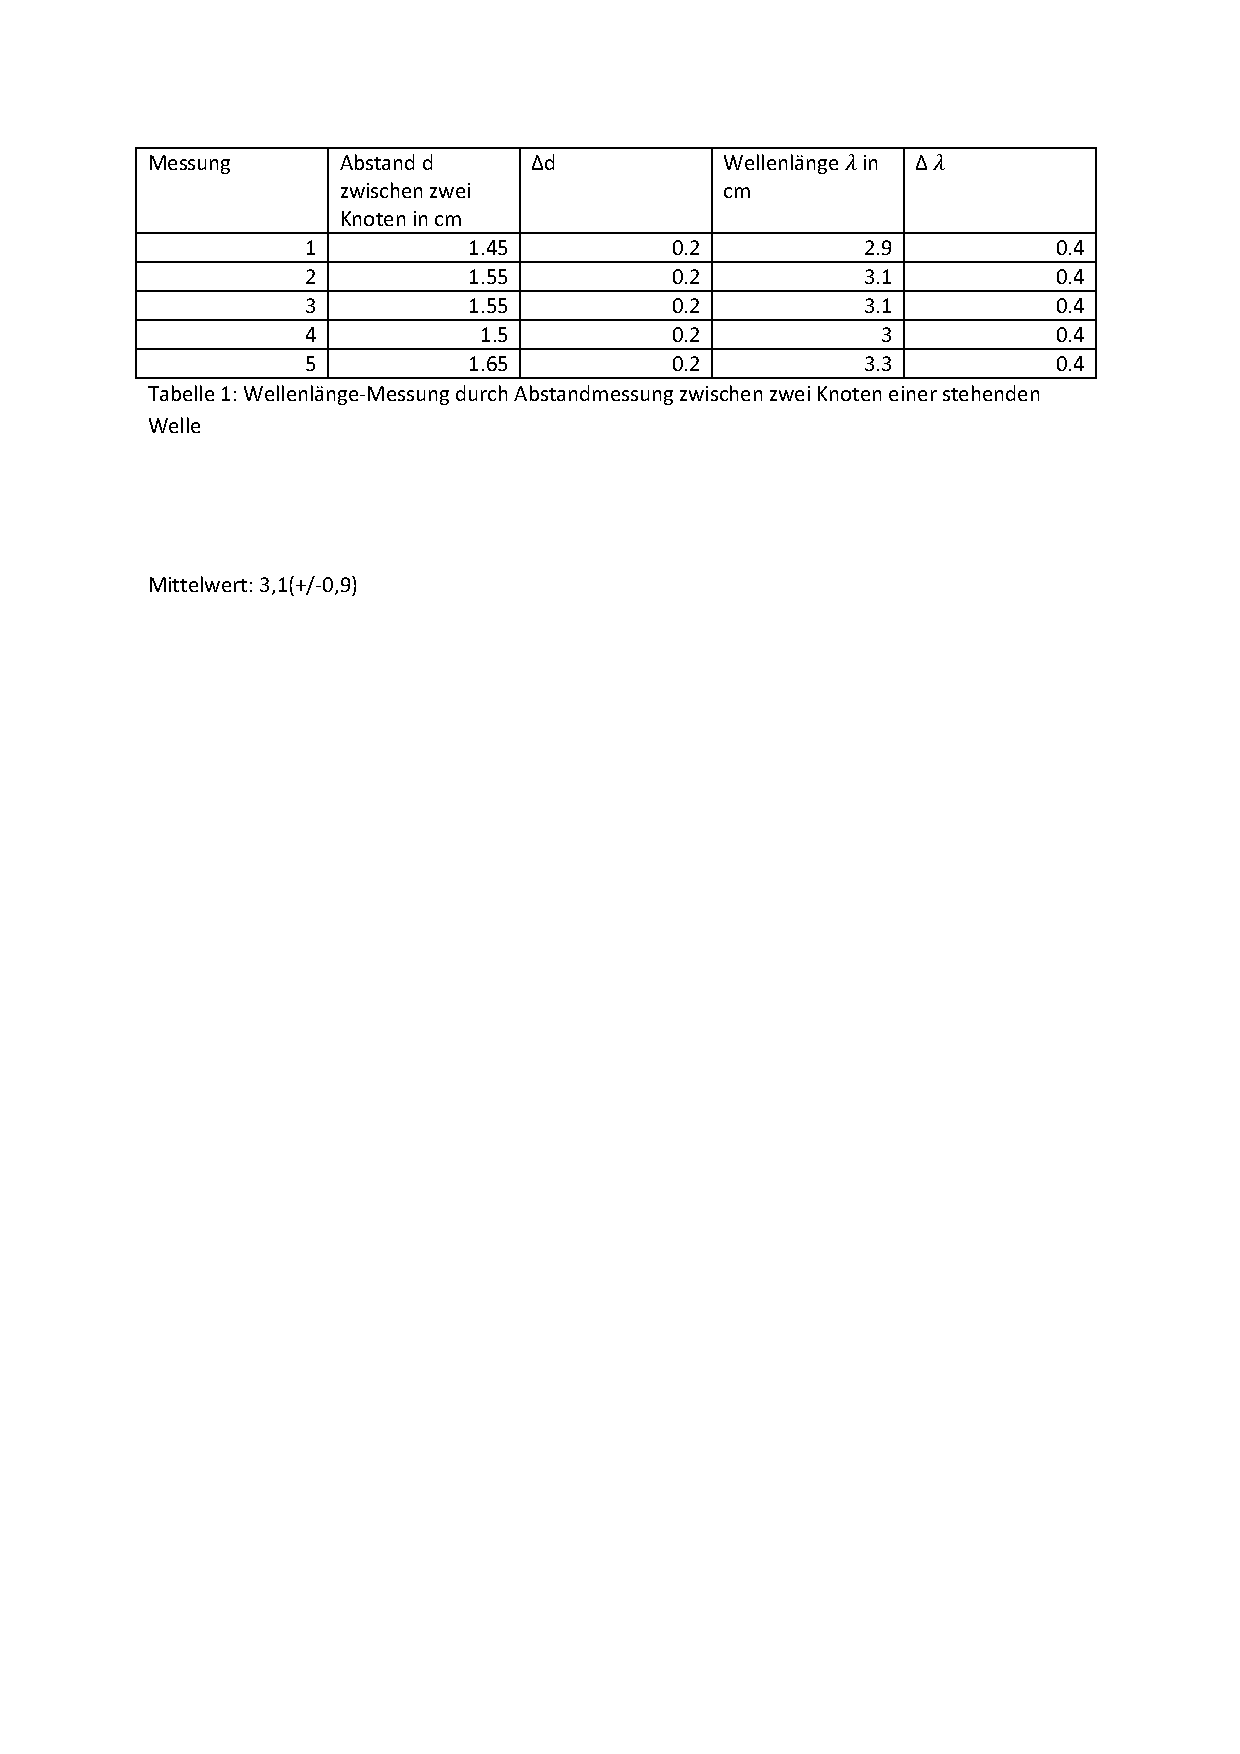
\includegraphics[width=\linewidth, trim=2.2cm 23.2cm 2.2cm 2.3cm, clip=true]{res/Nr3.pdf}
\caption{Wellenlänge-Messung durch Abstandsmessung zwischen zwei Knoten einer stehenden Welle.}
\label{fig:wellenl}
\end{table}
Aus dem Mittelwert bekommen wir $\lambda=\SI{3.08(15)}{cm}$.

\subsection{Brechungsindex von PVC für Mikrowellen}
Die flache Seite eines PVC-Halbzylinders wurde aus fünf verschiedenen Einfallswinkeln $\vartheta_1$ mit Mikrowellen beleuchtet und jeweils der Transmissionswinkel $\vartheta_2$ gemessen. Dazu wurde der Empfänger auf der dem Sender gegenüberliegenden Seite des Halbzylinders bewegt, bis ein Spannungsausschlag verzeichnet wurde.
\begin{table}[h]
\centering
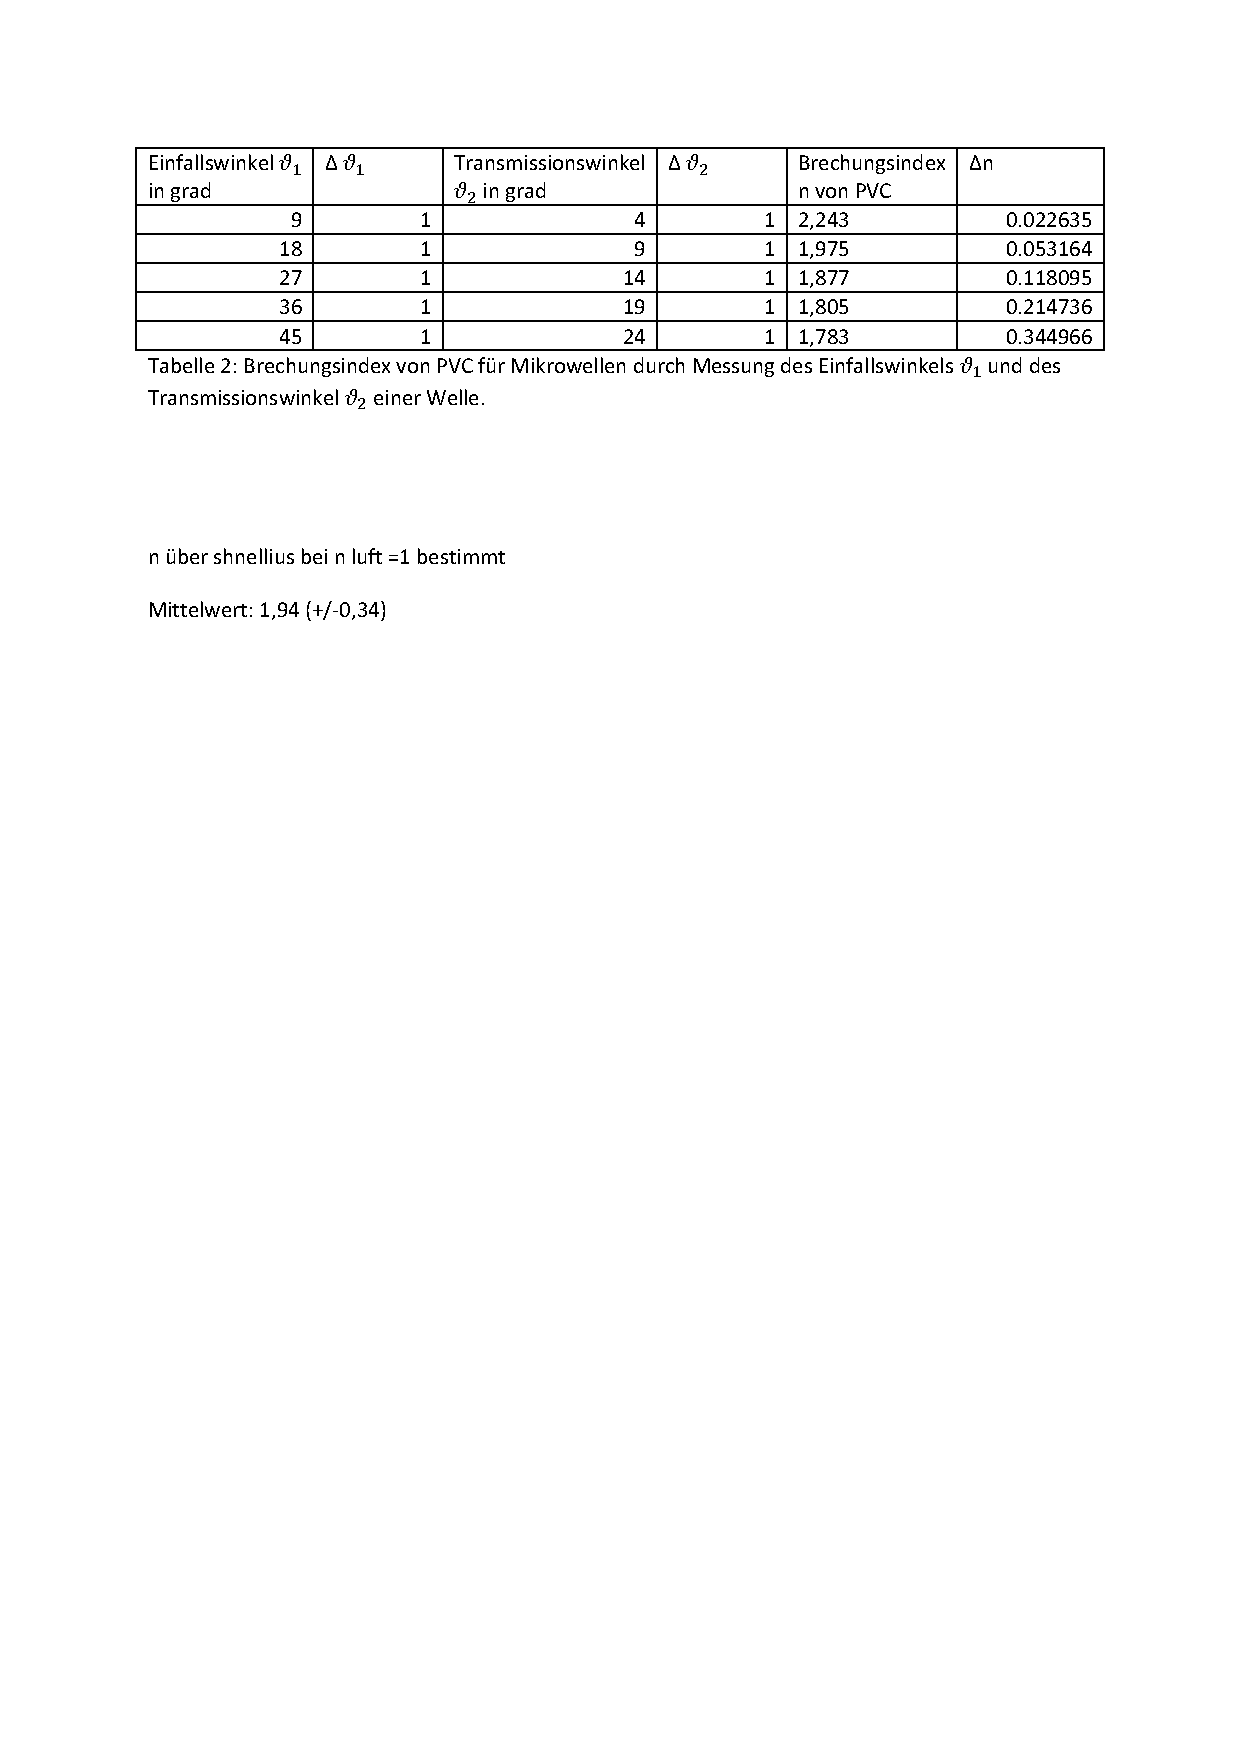
\includegraphics[width=\linewidth, trim=2.2cm 23.7cm 2.2cm 2.3cm, clip=true]{res/Nr4.pdf}
\caption{Brechungsindex von PVC für Mikrowellen durch Messung des Einfallswinkels $\vartheta_1$ und des Transmissionswinkels $\vartheta_2$ einer Welle.}
\label{fig:brech}
\end{table}
Der Brechungsindex wurde aus dem Snelliusschen Brechungsgesetz (\cref{eq:snellius}) bestimmt, wobei für Luft $n_1=1$ angenommen wurde. Der Mittelwert ist $n_{\text{PVC}}=\num{1.94(34)}$.

\subsection{Totalreflexion}
Nun wurde die runde Seite des PVC-Halbzylinders bestrahlt und der Einfallswinkel solange abgeflacht, bis keine transmittierte Welle mehr gemessen wurde. Nachdem die Totalreflexion erreicht war, wurde ein zweiter PVC-Halbzylinder hinter den ersten gebracht und mit dem Empfänger die transmittierte Welle gesucht. Anschließend wurde die Intensität der transmittierten Welle bei verschiedenen Abständen zwischen den Halbzylindern gemessen.
\begin{figure}[H]
\centering
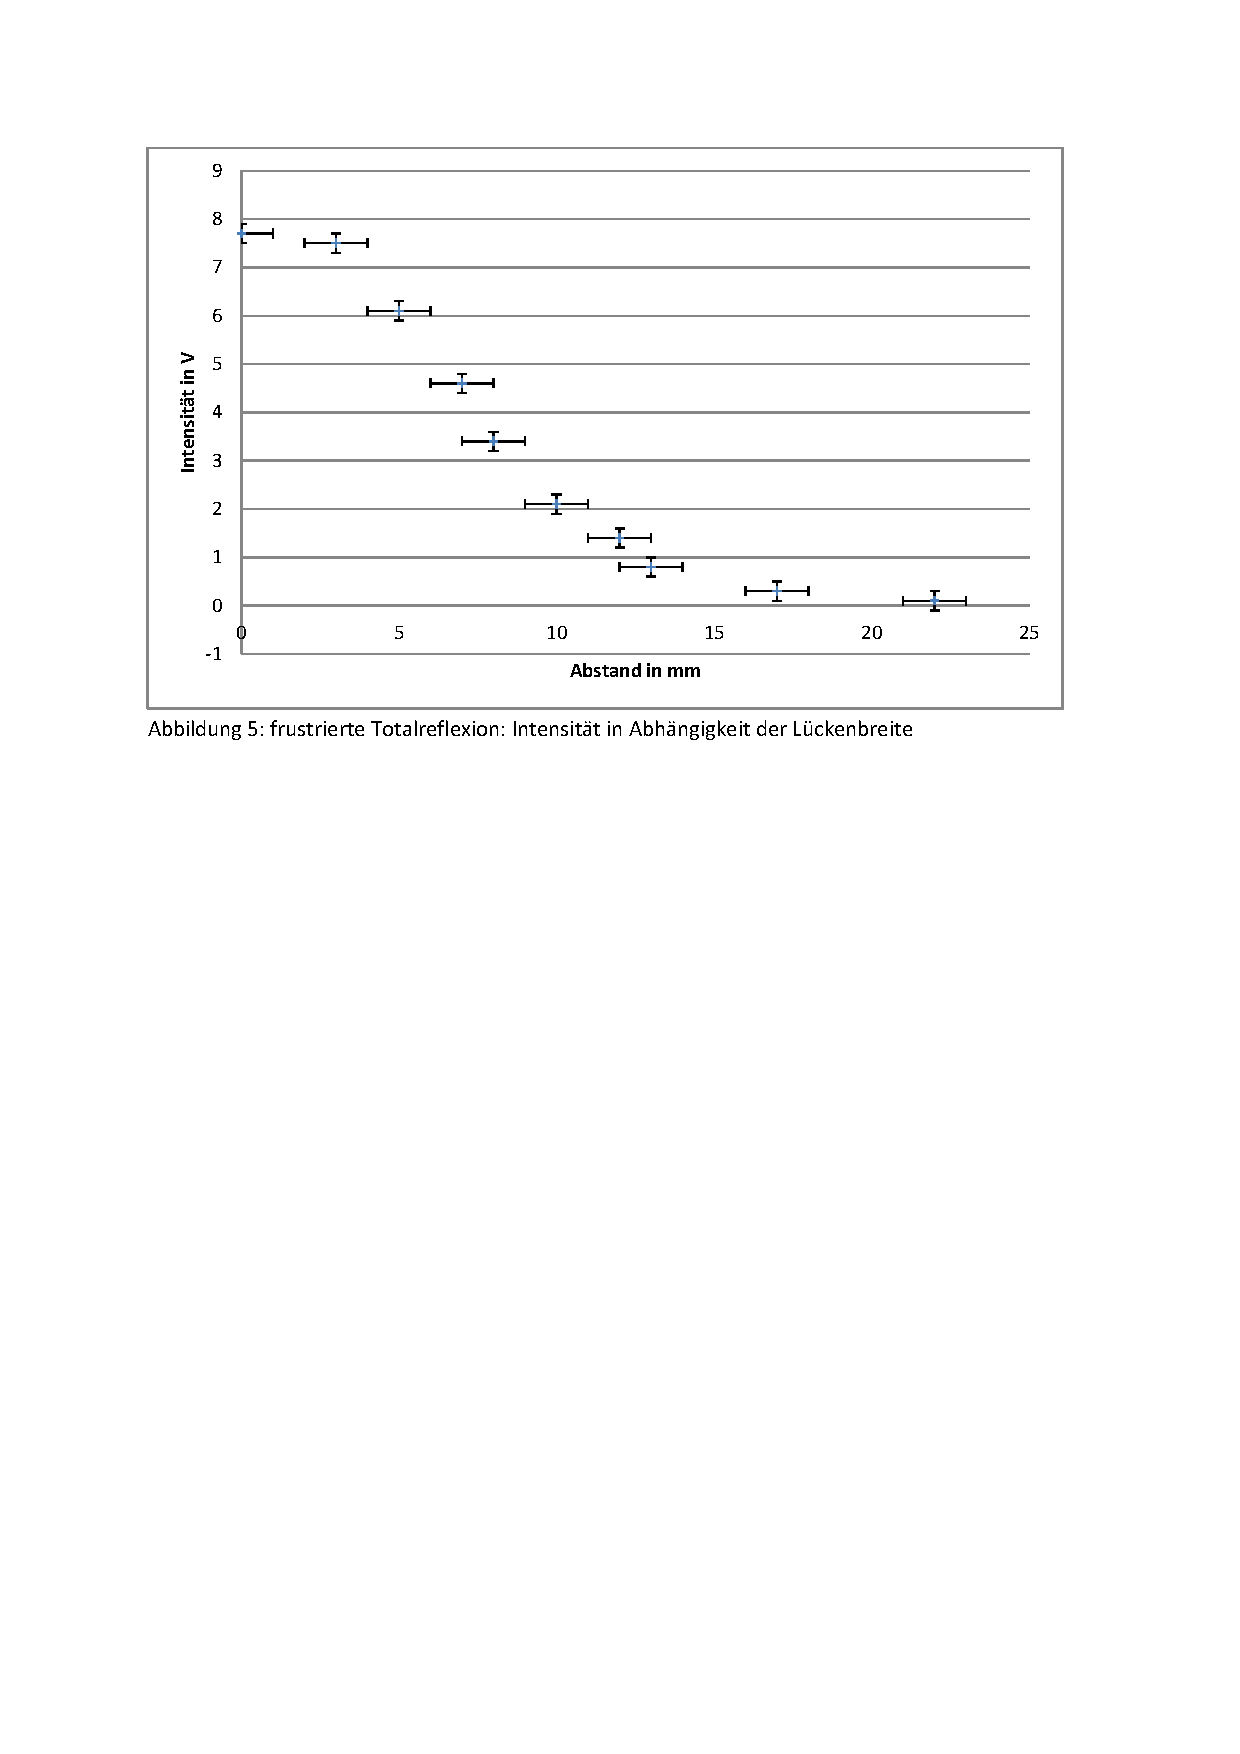
\includegraphics[width=\linewidth, trim=2.2cm 17.6cm 2.2cm 2.3cm, clip=true]{res/Nr5.pdf}
\caption{Frustrierte Totalreflexion: Intensität in Abhängigkeit der Lückenbreite.}
\label{fig:frustriert}
\end{figure}

\subsection{Bragg-Reflexion}
Ein Schaumstoffquader mit einem Gitter aus Metallkugeln, die zueinander den Abstand $d$ haben, wurde in den Strahlengang gebracht. 
Abhängig vom Einfallswinkel wird die Intensität der reflektierten Welle (mit Ausfallswinkel=Einfallswinkel) gemessen.
\begin{figure}[H]
\centering
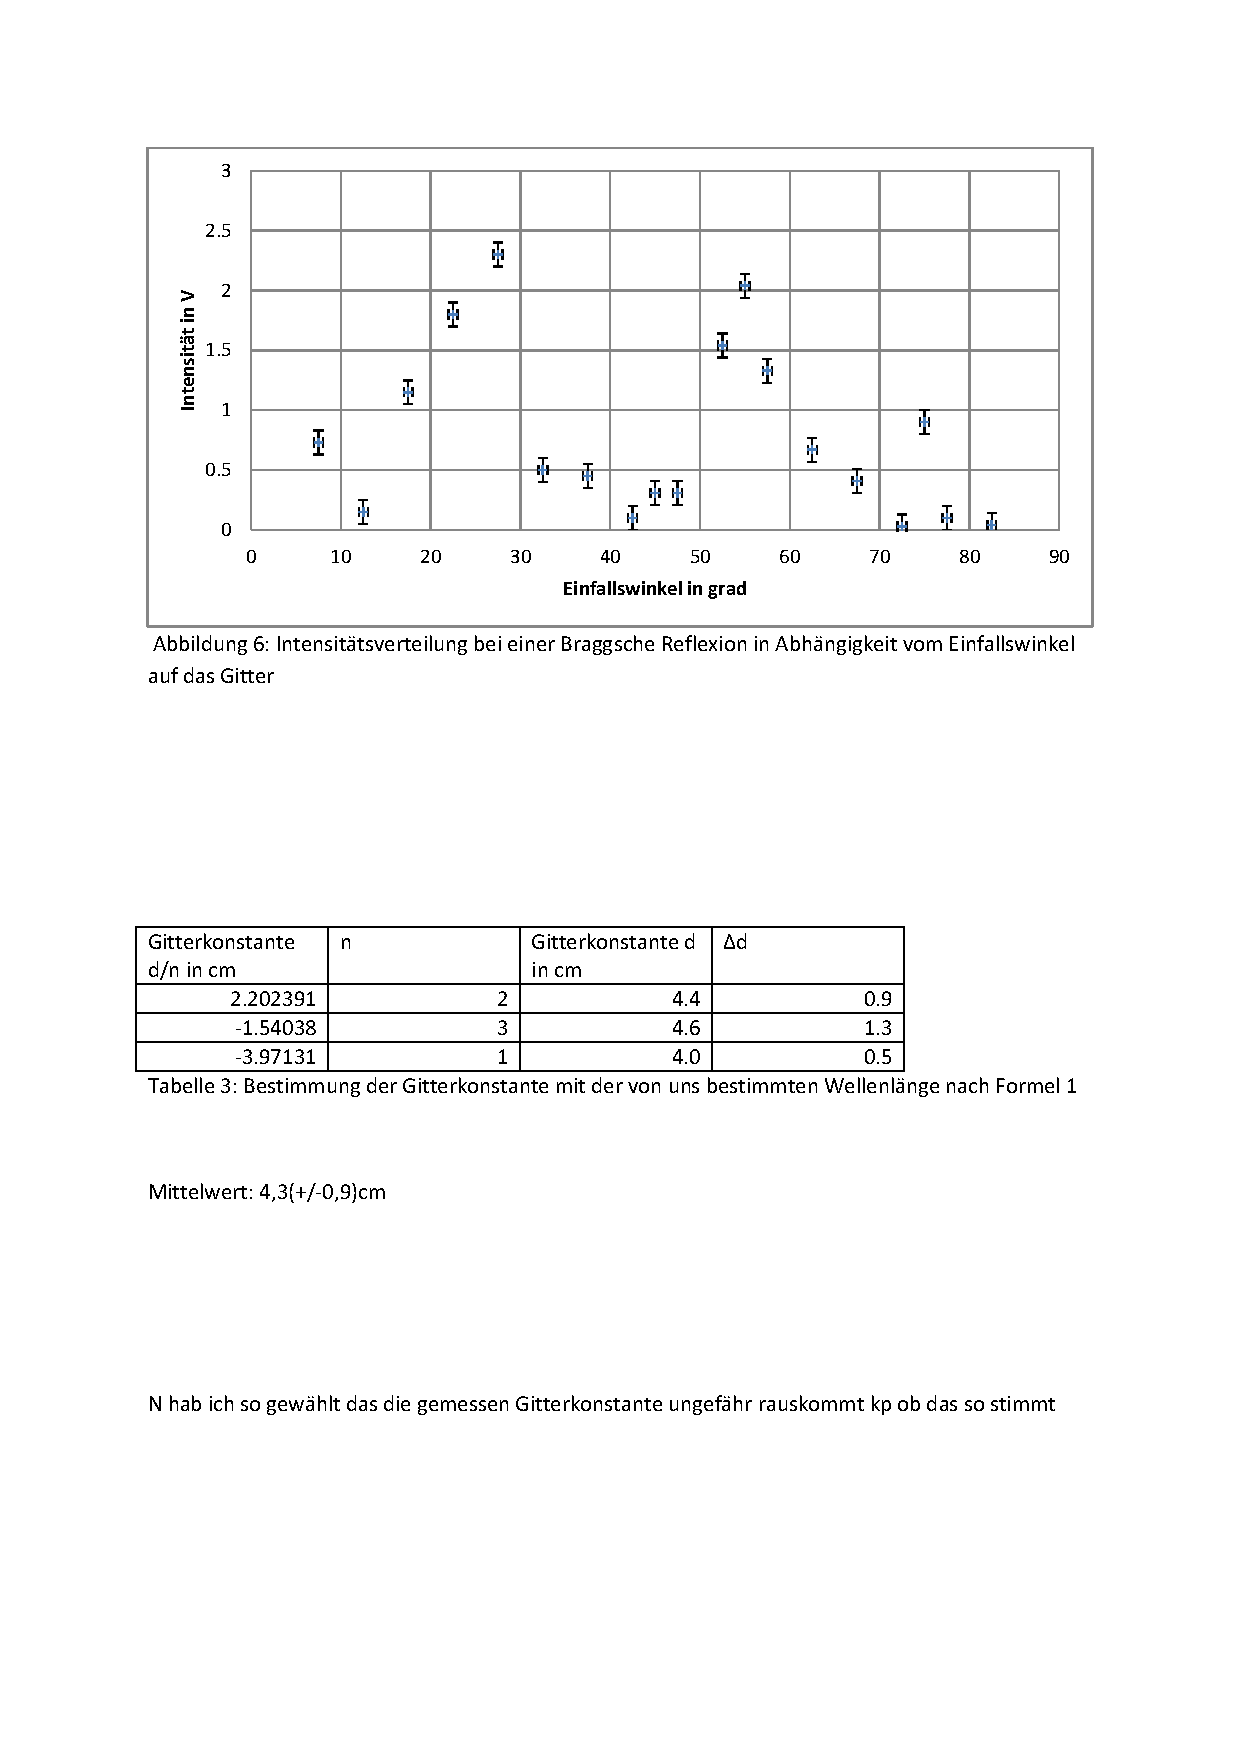
\includegraphics[width=\linewidth, trim=2.2cm 19cm 2.3cm 2.3cm, clip=true]{res/Nr6.pdf}
\caption{Intensitätsverteilung bei einer Bragg-Reflexion in Abhängigkeit vom Einfallswinkel auf das Gitter.}
\label{fig:bragg}
\end{figure}
Die Maxima werden abgelesen und mithilfe von \cref{eq:bragg} die Gitterkonstante bestimmt.
\begin{table}[H]
\centering
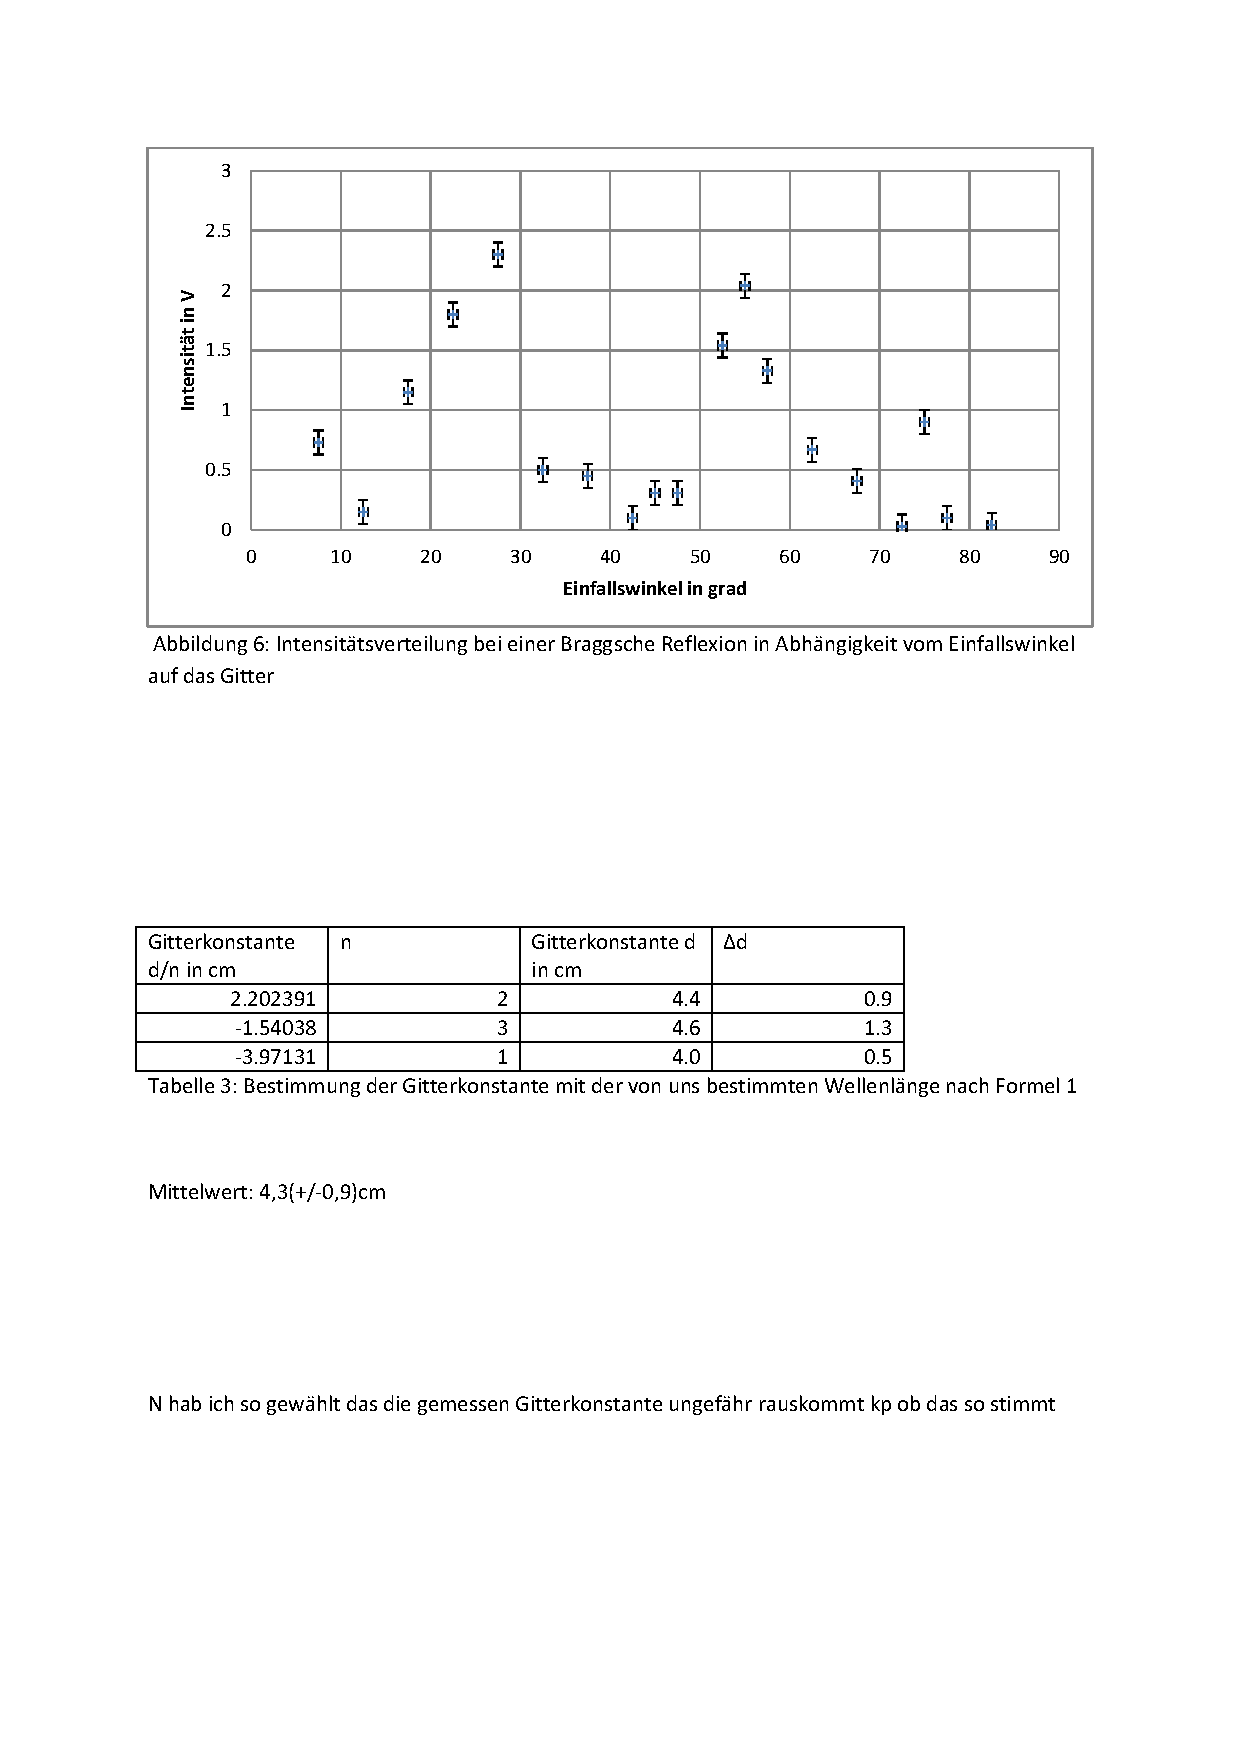
\includegraphics[width=\linewidth, trim=2.2cm 11.5cm 5.6cm 15.6cm, clip=true]{res/Nr6.pdf}
\caption{Bestimmung der Gitterkonstante mit der von uns bestimmten Wellenlänge nach \cref{eq:bragg}.}
\label{tab:bragg}
\end{table}

Heraus kommt als Mittelwert $d=\SI{4.3(9)}{cm}$.
\section{Diskussion}
Bei der Bestimmung der Strahldivergenz war wie erwartet ein linearer Zusammenhang zwischen Abstand zum Sender und Aufweitung des Strahls zu sehen. Der virtuelle Quellfleck lag fast auf der optischen Achse. Die Abweichung ist auf eine leicht schiefe Stellung von Sender oder Empfänger zurückzuführen. 

Der Quellfleck lag \SI{9.82}{cm} vor dem Sender. Hier ist zu beachten, dass der Abstand bezüglich der hinteren Wand des Senders gemessen wurde. Davor war ein Trichter angebracht, der den Strahl verformt haben könnte.\\

Die Wellenlänge konnte mit der Methode der stehenden Wellen mit geringem Fehler zu $\lambda=\SI{3.08(15)}{cm}$ bestimmt werden. Dies liegt tatsächlich im Bereich der Mikrowellen (vgl. Einführung).

Bei der Bestimmung des Brechungsindex von PVC fällt auf, dass für spitzere Winkel ein größerer Wert gemessen wurde. Möglicherweise liegt dies an der Strahldivergenz, da die einfallende Welle in der Realität nicht kollimiert ist.\\

In \cref{fig:frustriert} konnte die evaneszente Welle über die frustrierte Totalreflexion mit dem zweiten Halbzylinder nachgewiesen werden. Zu sehen ist außerdem die exponentielle Abnahme mit zunehmendem Abstand.\\

Bei der Bragg-Reflexion konnten drei Maxima nachgewiesen werden. Über die vorher bestimmte Wellenlänge wurde die Gitterkonstante zu $d=\SI{4.3(9)}{cm}$ bestimmt. Der Fehler ist groß, da die genaue Position der Maxima schlecht abzulesen ist. Mit einem Geodreieck wurde $d=\SI{3.8(1)}{cm}$ nachgemessen, was gut mit dem Wert aus der Bragg-Reflexion übereinstimmt.

\nocite{anleitung-ss2015}